\section{Instrumentation}
\label{sec:afm}

Of the mechanical manipulation methods listed in
\cref{sec:single-molecule}, AFM is the most widely used due to the
availability of user-friendly commercial instruments.  AFM has been
employed on several types of biological macromolecules, mechanically
unfolding proteins\citep{carrion-vazquez99a} and forcing structural
transitions in DNA\citep{florin95,rief99} and
polysaccharides\citep{rief97a}.

An AFM\index{AFM} uses a sharp tip integrated at the end of a
cantilever to interact with the sample\citep{binnig86}.  Cantilever
bending is measured by a laser reflected off the cantilever and
incident on a position sensitive photodetector\citep{meyer88}
(\cref{fig:afm-schematic}).  When the bending force constant of the
cantilever is known\citep{levy02}, the force applied to the sample can
be calculated using Hooke's law (\cref{eq:sawsim:hooke}).

The substrate is mounted in a fluid cell\citep{drake89,radmacher92} on
a three dimensional piezoelectric actuator so that the tip may be
positioned on the surface with sub-nanometer resolution (although
signal drift and piezo hysteresis can cause larger errors in the
positioning accuracy).  Our tubular piezo has a range of
$1.6\U{$\mu$m}$ in the horizontal directions and a range of
$3.5\U{$\mu$m}$ in the vertical (\cref{fig:piezo-schematic}).

\begin{figure}
  \begin{center}
    \subfloat[][]{\label{fig:afm-schematic}
      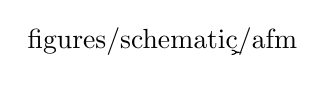
\begin{tikzpicture}[remember picture]
        \node[anchor=south west,inner sep=0] (image) at (0,0) {
          \asyinclude{figures/schematic/afm}};
        \begin{scope}[x={(image.south east)},y={(image.north west)}]
          \draw [decorate,decoration={brace,raise=4pt,mirror}]
              (0.715,0.05) -- (0.715,0.2)
              node [midway,xshift=3pt] (afm-piezo-brace) {};
        \end{scope}
      \end{tikzpicture}
    }
    \hspace{.25in}%
    \subfloat[][]{\label{fig:piezo-schematic}
      \begin{tikzpicture}[remember picture]
        \node[anchor=south west,inner sep=0] (image) at (0,0) {
          \asyinclude{figures/schematic/piezo}};
        \begin{scope}[x={(image.south east)},y={(image.north west)}]
          \draw [decorate,decoration={brace,raise=4pt}]
              (0,0.1) -- (0,0.9)
              node [midway,xshift=-3pt] (piezo-brace) {};
          \draw [overlay,out=0,in=180] (afm-piezo-brace) to (piezo-brace);
        \end{scope}
      \end{tikzpicture}
    }
    \caption{\protect\subref{fig:afm-schematic} Operating principle
      for an Atomic Force Microscope\index{AFM}.  A sharp tip
      integrated at the end of a cantilever interacts with the sample.
      Cantilever bending is measured by a laser reflected off the
      cantilever and incident on a position sensitive photodetector.
      \protect\subref{fig:piezo-schematic} Schematic of a tubular
      piezoelectric actuator.  In our AFM, the substrate is mounted on
      the top end of the tube, and the bottom end is fixed to the
      microscope body.  This allows the piezo to control the relative
      position between the substrate and the AFM cantilever.  The
      electrodes are placed so radial electric fields can be easily
      generated.  These radial fields will cause the piezo to expand
      or contract axially.  The $z$ voltage causes the tube to expand
      and contract uniformly in the axial direction.  The $x$ and $y$
      voltages cause expansion on one side of the tube, and
      contraction (because of the reversed polarity) on the other side
      of the tube.  This tilts the tube, shifting the sample
      horizontally.\label{fig:afm-schematic-and-piezo}}
  \end{center}
\end{figure}

% really, AFM can do this ;)
The forces that can be applied and measured with an AFM range from
tens of piconewtons to hundreds of nanonewtons.  The investigation of
the unfolding and refolding processes of individual protein molecules
by the AFM is feasible because many globular proteins unfold under
external forces in this range.  Since elucidating the mechanism of
protein folding is currently one of the most important problems in
biological sciences, the potential of the AFM for revealing
significant and unique information about protein folding has
stimulated much effort in both experimental and theoretical research.
